% Chapter Template

\chapter{Ensayos y resultados} % Main chapter title

En este capítulo se describen los ensayos realizados, se comentan las herramientas que se utilizaron y se presentan los resultados.

\label{Chapter4} % Change X to a consecutive number; for referencing this chapter elsewhere, use \ref{ChapterX}

%----------------------------------------------------------------------------------------
%	SECTION 1
%----------------------------------------------------------------------------------------

\section{Generación del sistema de pruebas}
\label{sec:pruebasHW}

En esta sección se explica cómo se hicieron los ensayos, qué resultados se obtuvieron, se presenta su análisis y se contrasta con los requerimientos.

\section{Pruebas unitarias}
En esta sección se presentan las herramientas que se utilizaron para ensayar las distintas partes del sistema en forma separada.

\subsection{Pruebas del servidor Mosquitto}
Para simular mensajes y observar el comportamiento de cada una de las partes del sistema se utilizó la herramienta MQTT explorer   \citep{WEBSITE:29}.

\begin{figure}[ht]
	\centering
	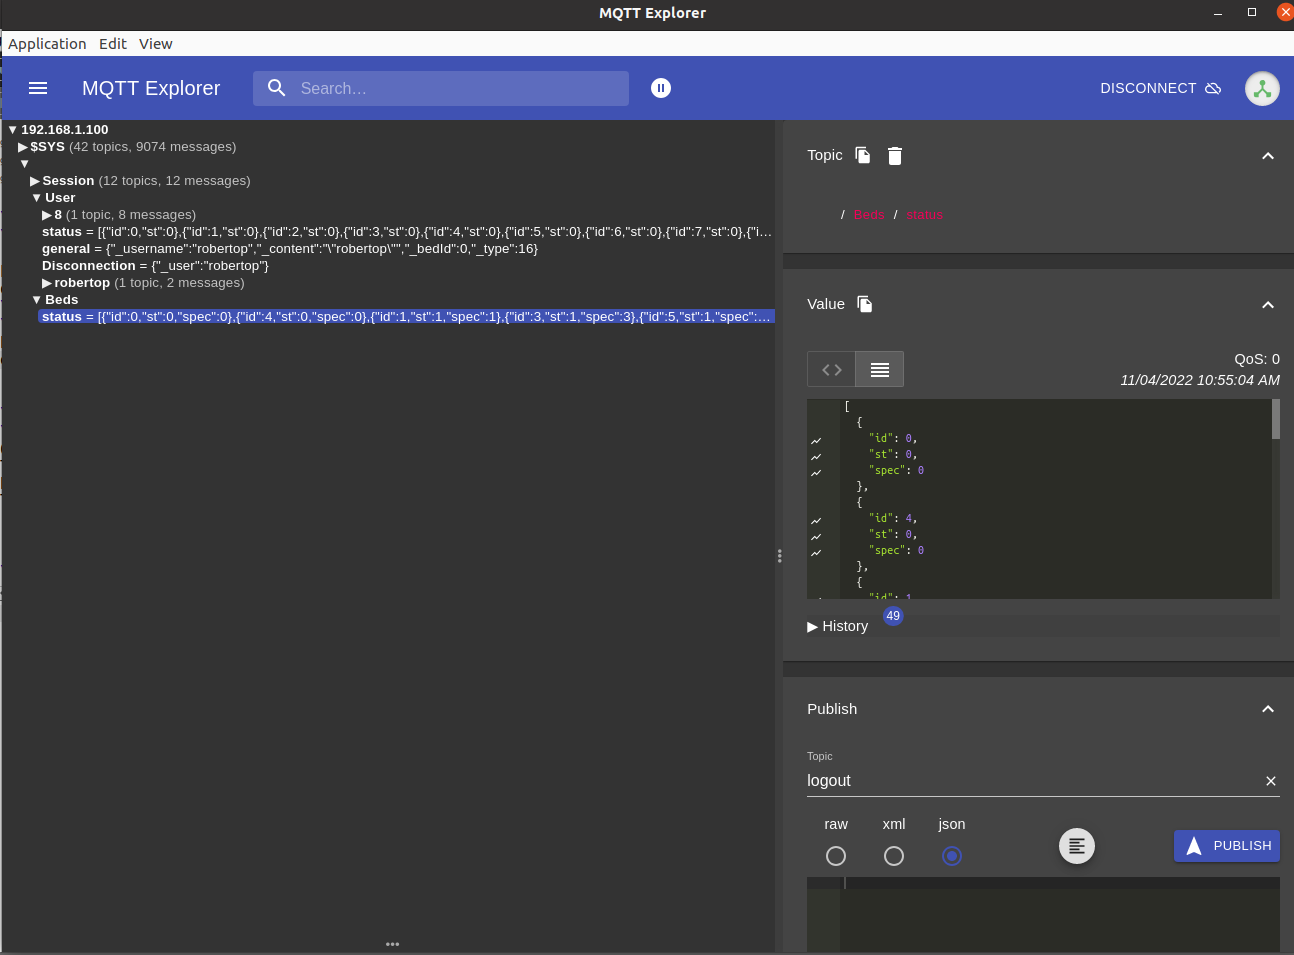
\includegraphics[scale=.25]{./Figures/mqtt-explorer.png}
	\caption{Imagen de MQTT Explorer.}
	\label{fig:MQTT Explorer}
\end{figure}

Esta herramienta fue importante no solo para realizar ensayos sino tambien para el desarrollo de las funcionalidades propiamente dichas.

\pagebreak

\subsection{Pruebas unitarias de la API Rest}

Para simular el logeo y la consulta a la base de datos se utilizó la herramienta PostMan \citep{WEBSITE:30}, Newman \citep{WEBSITE:35} y la consola de administrador de phpMyAdmin mencionada en \ref{subsec: Bases de datos relacionales}. En la figura \ref{fig:Logueo en el sistema con Postman} se observa el \textit{token} devuelto por el backend al logearse con las credenciales correspondientes y en \ref{fig:Rechazo Logueo en el sistema con Postman} se observa la respuesta al ingresar una contraseña inadecuada.

\begin{figure}[ht]
	\centering
	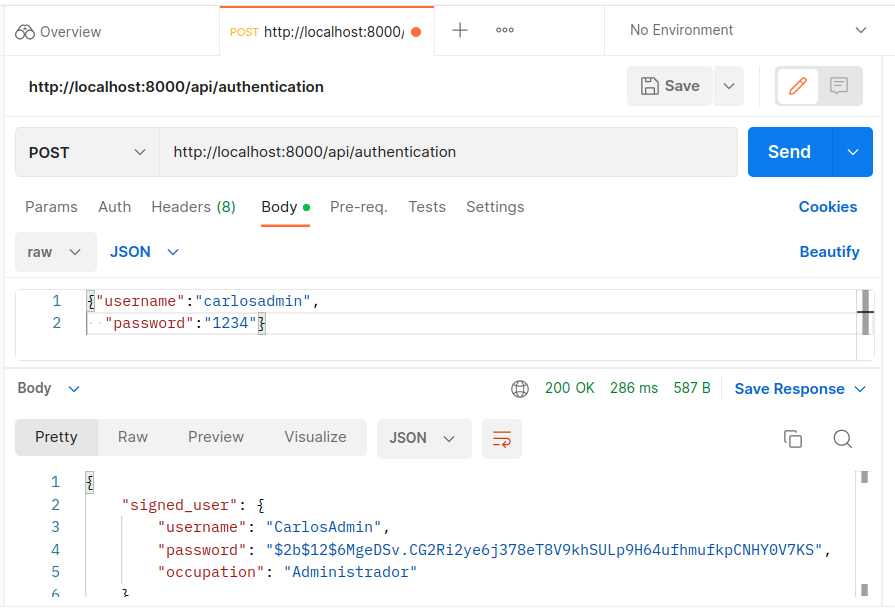
\includegraphics[scale=.35]{./Figures/auth.png}
	\caption{Logueo en el sistema con Postman.}
	\label{fig:Logueo en el sistema con Postman}
\end{figure}

\begin{figure}[ht]
	\centering
	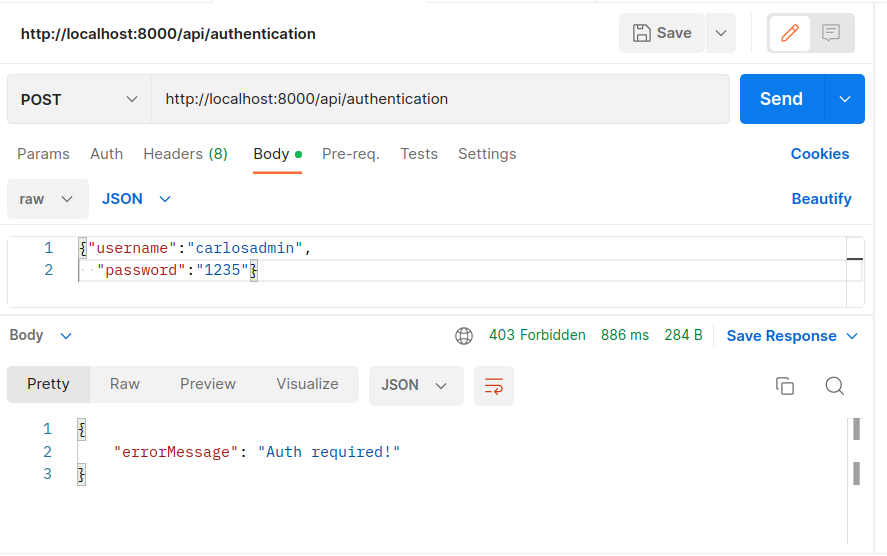
\includegraphics[scale=.35]{./Figures/no-auth.png}
	\caption{Rechazo de logueo.}
	\label{fig:Rechazo Logueo en el sistema con Postman}
\end{figure}

Postman permite automatizar los test utilizando colecciones (que son secuencias de consultas a la API). Las colecciones se pueden exportar a un formato JSON de modo de poder ser utilizadas por otras herramientas. En un entorno de integración continua y entrega continua, una herramienta de testeo automático permite, una vez definidos las colecciones de test, volver a ejecutarlos luego de haber realizado una modificación y obtener un resultado de los mismos, asegurando que no se modificó lo que ya funcionaba y que las mejoras pasen los nuevos test. 

Para utilizar Newman, que es el cliente de consola, se deben exportar las colecciones y luego utilizar la linea de comandos con dicha colección (ver figura \ref{fig:Colección logueo usuario en Postman}). 


\begin{figure}[ht]
	\centering
	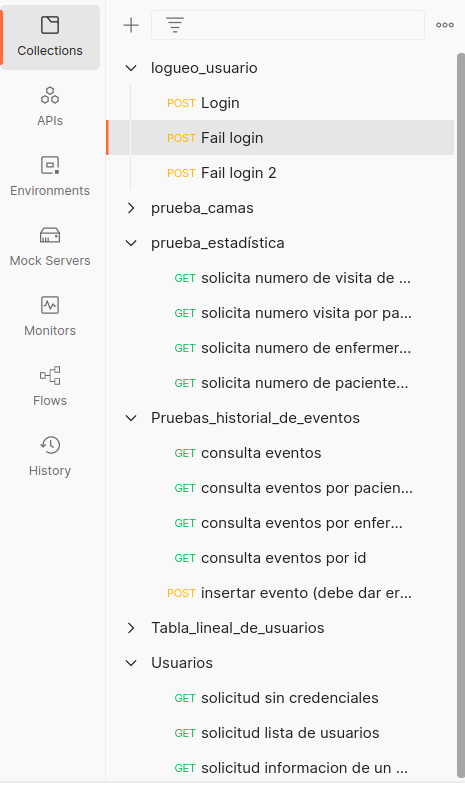
\includegraphics[scale=.25]{./Figures/Postman.png}
	\caption{Colección logueo de test.}
	\label{fig:Colección logueo usuario en Postman}
\end{figure}

Para reportar con Newman existen varias opciones, en este trabajo se utiliza cli y htmlextra, ejecutando en la consola:



\begin{lstlisting}[label=cod:Newman,caption=  Ejecución de Newman en consola]
>>newman run ./logueo_usuario.postman_collection.json -r cli,htmlextra
\end{lstlisting}



En la figura \ref{fig:reporte cli Newman} se observa el reporte por consola y en \ref{fig:reporte html Newman} el reporte en html.

\begin{figure}[ht]
	\centering
	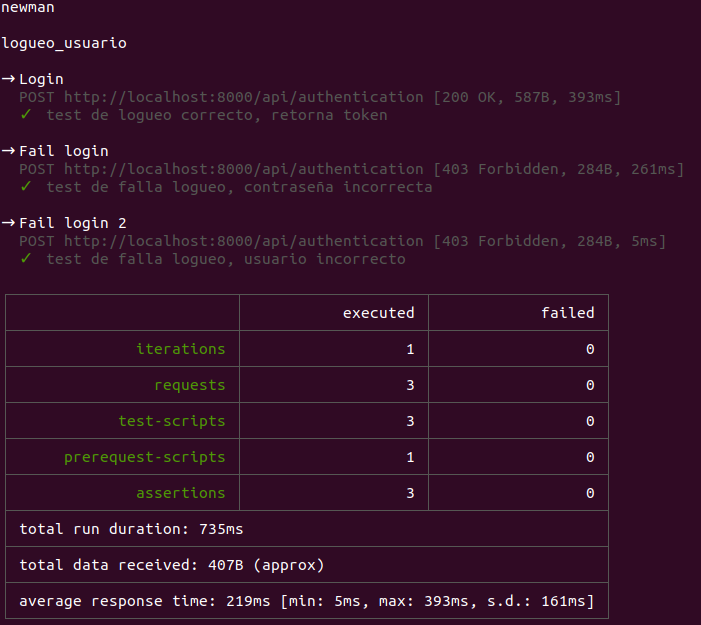
\includegraphics[scale=.35]{./Figures/newman-1.png}
	\caption{Reporte en consola de Newman.}
	\label{fig:reporte cli Newman}
\end{figure}


\begin{figure}[ht]
	\centering
	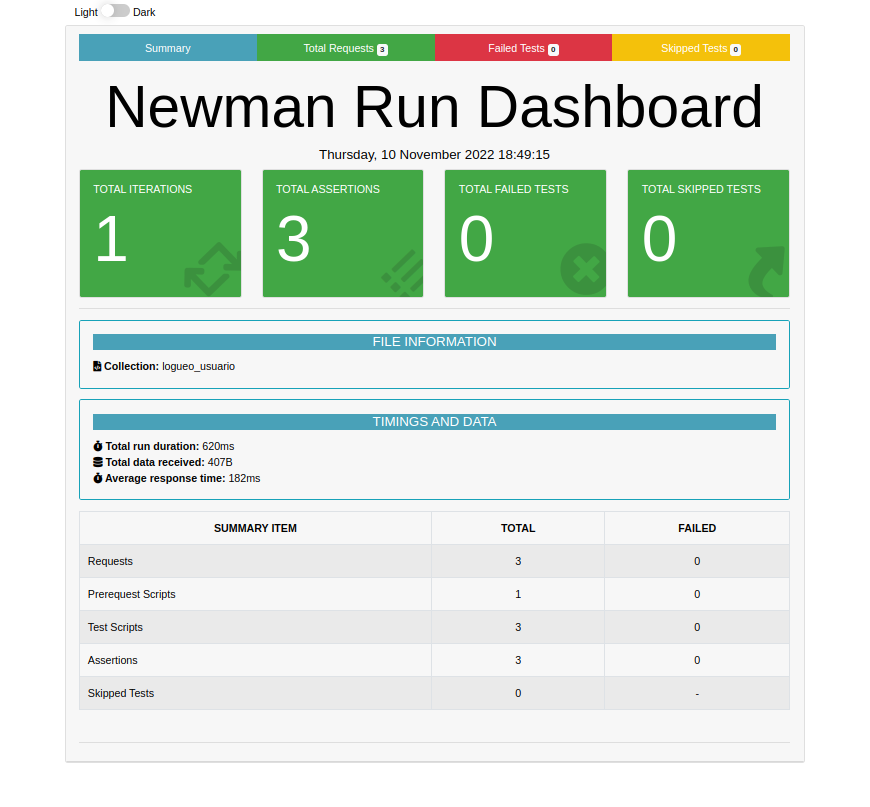
\includegraphics[scale=.35]{./Figures/newman-2.png}
	\caption{Reporte html de Newman.}
	\label{fig:reporte html Newman}
\end{figure}

\pagebreak

\section{Integración del sistema}
\label{Integración del sistema}

En esta sección se comenta como se instaló el backend y el servidor web en una máquina remota, se instaló la aplicación en múltiples dispositivos, se desarrollo un dispositivo que simula los eventos de los llamadores de los hospitales, se ensayo el sistema durante una semana y se analiza los resultados de la simulación de uso.

Se utilizó como máquina remota una instancia en Amazon Web Services y los dispositivos móviles en los cuales se instalo el dispositivos, fueron celulares con el sistema Android como sistema operativo.

\subsection{Instalación del sistema en una instancia de AWS}
Con el objetivo de no incorporar costos en las pruebas, se generó una instancia Free Tier en Amazon Web Services, en la cual se instaló Ubuntu, el broker Mosquitto, el backend, la página Web y un servidor NGINX para que funcione como proxy reverso. Tambien se contrató el servicio route 53 que permite personalizar las politicas de ruteo.
De esta manera, se puede acceder al sistema desde cualquier dispositivo móvil conectado a una red.
Los pasos para configurar el sistema backend en la instancia EC2 con ubuntu son:

\begin{enumerate}


\item Logearse en la instancia con ssh.
\item Instalar Git:

	''sudo apt-get install git''
\item Instalar el broker Mosquitto:
	
	''sudo apt-get install mosquitto''
\item Configurar el brocker Mosquitto según sección \ref{Broker Mosquitto}.
\item Instalar Docker y Docker-compose
\item Descargar el backend desde GitHub
\item Copiar en la instancia la base de datos comprimida y descomprimir dentro de la carpeta /db
\item Ejecutar Docker-compose up
\end{enumerate}

Los pasos para configurar la página web:
\begin{itemize}
\item Compilar la página web: dentro del proyecto ejecutar:

''ionic build''
\item Comprimir la carpeta www
\item Logearse con ssh en la instancia EC2
\item configurar nginx para redirigir a la página (ver apéndice \ref{AppendixB}).

\end{itemize}
\subsection{Generación/instalación de la aplicación móvil en Android}

Para que la aplicación pueda utilizarse en un dispositivo móvil, la misma debe ser compilada para ejecutarse en código nativo. Con esto se genera el código instalable .apk para Android y .ipa para IOS. La distribución segura de las aplicaciones se realiza a través de los  

Para poder descargar el archivo ejecutable a un dispositivo Android se debe generar el archivo .apk correspondiente. Para ello seguir los siguientes pasos:

\begin{itemize}
\item Generar código con ionic capacitor:

''ionic cap build android''
\item Abrir Android estudio, modificar el AndroidManifest.xml
\item Generar el bundle o en su defecto, conectar el celular en modo debug y descargar la aplicación (ver apéndice \ref{AppendixA}).
\end{itemize}
\pagebreak


\begin{lstlisting}[label=cod:AndroidMan,caption=Modificaciones al Android Manifest.]  % Start your code-block

package="com.gabiot.Enfermera">
    <!-- Permissions -->

    <uses-permission android:name="android.permission.INTERNET" />
    <uses-permission android:name="android.permission.READ_EXTERNAL_STORAGE" />
    <uses-permission android:name="android.permission.WRITE_EXTERNAL_STORAGE" />
    <uses-permission android:name="android.permission.ACCESS_NETWORK_STATE" />
    <uses-permission android:name="android.permission.ACCESS_WIFI_STATE" />

    <uses-permission android:name="android.permission.WAKE_LOCK" />
    <uses-permission android:name="android.permission.READ_PHONE_STATE" />
    <uses-permission android:name="android.permission.CAMERA" />
    <uses-sdk tools:overrideLibrary="com.google.zxing.client.android" />
    <uses-permission android:name="android.permission.RECORD_AUDIO" />

    <application
        android:allowBackup="true"
        android:icon="@mipmap/ic_launcher"
        android:label="Enfermera"
        android:roundIcon="@mipmap/ic_launcher_round"
        android:supportsRtl="true"
        android:theme="@style/AppTheme"
        android:usesCleartextTraffic="true"
        android:hardwareAccelerated="true">
        <!-- Mqtt Service -->
        <service
            android:enabled="true"
            android:name="org.eclipse.paho.android.service.MqttService"
            android:exported="false"
        />
...

\end{lstlisting}
\pagebreak
\subsection{Equipo simulador de llamadores}

Se desarrollo un dispositivo que simula los llamadores con un microcontrolador ESP32, una fuente y un teclado matricial. Presionando una tecla, genera un evento en MQTT. El código y el esquemático del mismo se encuentra en \citep{WEBSITE:33}. 

\begin{figure}[ht]
	\centering
	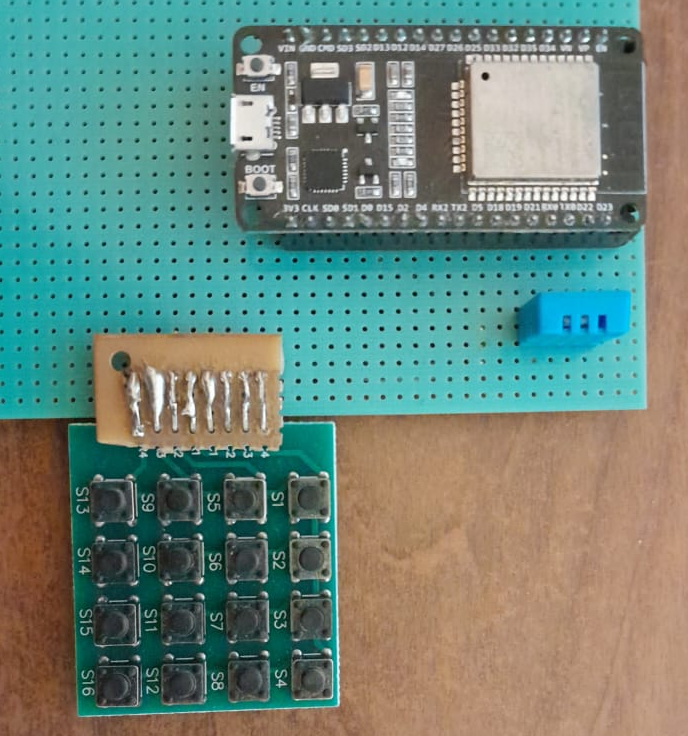
\includegraphics[scale=.35]{./Figures/simulador.png}
	\caption{Simulador de llamadores.}
	\label{fig:Simulador de llamadores}
\end{figure}

\subsection{Resultados de utilizar el sistema}
\label{Resultados de utilizar el sistema}
El sistema permaneció funcionando de manera adecuada durante una semana completa, generando los eventos programados y permitiendo la interacción de dispositivos.
\pagebreak
\section{Contraste con los requerimientos}
\label{Contraste con los requerimientos}

En esta subsección se detalla el grado de cumplimiento de los requerimientos relevados en el plan de proyecto.
\begin{enumerate}
\item Requerimientos del servidor: 

1.1 debe tener instalado el broker mosquitto.

Verificación: Se muesta el funcionamiento del servidor utilizando la aplicación MQTT explorer.

\item Requerimientos de la base de datos: 

2.1 Debe poseer una base de datos relacional. 

2.2 Debe poseer las siguientes tablas: eventos, pacientes, médicos, enfermeras. 

2.2 La base de datos debe poseer datos cargados por default.

Verificación: Se muesta el contendio de la base de datos con la aplicación phpMyAdmin.

\item Requerimientos de la página web 

3.1 Debe ser cliente del broker MQTT. 

Verificación: Se presenta la configuración del broker. Se presenta el monitoreo de las habitaciones y los usuarios conectandose al broker.

3.2 La página debe poseer funciones de consulta o modificación de la base de datos.

Verificación: Se muestra como la página web permite cambiar contraseñas de usuarios y otros parámetros.

3.3 La página debe permitir observar estadística de pacientes y enfermeras.

Verificación: Se muestra como la página web permite observar distintas gráficas.

3.4 La página debe contener acceso con usuario y contraseña para cada persona.


Verificación: Se muestra como la página web permite loguear los distintos usuarios.
(*) Cumplimiento parcial: solo permite loguear al usuario administrador.

\item Requerimientos de la aplicación móvil

4.1 y 4.2 La aplicación debe poseer tres modos de uso: médico, enfermera y sistema. 

Verificación: Se ingresa a la aplicación en los distintos modos.

4.3 La aplicación en modo enfermera debe permitir leer código QR.

Verificación: Se ingresa a la aplicación en modo enfermera y siguiendo los pasos se obtiene el código QR.

4.4 La aplicación en modo enfermera debe descargar información relevante del paciente.

Verificación: Se ingresa a la aplicación en modo enfermera y siguiendo los pasos se descarga las notas del paciente.

4.5 La aplicación en modo sistema debe mostrar las habitaciones sin atención, según una tabla de prioridades y en caso de igualdad de prioridades mostrar según un orden de llamada.

(*)Cumplimiento parcial: se muestra las habitaciones con una tabla de prioridades pero no según el orden de llamadas.

Verificación: Se ingresa a la aplicación en modo enfermera y siguiendo los pasos se descarga las notas del paciente.


4.6 El modo de usuario médico y el modo usuario enfermera deben poder enviar mensajes de texto o sonido.

Verificación: Se transmiten distintos audios entre participantes.

\item Requerimientos de la documentación

5.1 Documento con información relativa a la base de datos: detalles de la misma y API para acceder.

Verificación: Se observa la presencia de la información en el repositorio de GitHub.

5.2 Memoria del proyecto con diagramas de aplicación móvil y página web.

Verificación: se verifica con este documento.

\item Requerimientos de la integración del sistema

6.1 El sistema debe integrar el funcionamiento del servidor con la base de datos, aplicación web y aplicaciones móviles.

Verificación: se verifico el funcionamiento en un laboratorio con 4 usuarios y un simulador de 8 llamadores durante una semana.

(*)Cumplimiento parcial:
Validación: No se pudo validar el sistema en un nosocomio.

\item Requerimientos de la entrega del producto:

7.1 El Código fuente del servidor debe ser subido a dockerhub y compartido con la comunidad.

(*)Cumplimiento parcial:
Validación: Se subió el código fuente del servidor a Github.

7.2 El Código fuente de la aplicación debe ser subido a GitHub y compartido con la comunidad.

Validación: Se subió el código fuente del servidor a Github.

\end{enumerate}
